% Dokumenteinstellungen und Anpassungen
\input{resources/settings/settings}
\input{resources/styles/adjustments}

\usepackage{graphicx}
\usepackage{subcaption}
\usepackage{float}
\usepackage{color}
\usepackage{listings}
\usepackage{eso-pic}
\usepackage[sf]{titlesec}
\usepackage{acronym}
\usepackage[normalem]{ulem}
%\usepackage[ngerman]{babel}
\usepackage{hyperref}
\usepackage{pdfpages}
\usepackage[toc,page]{appendix}


\addto\captionsnenglish{\let\appendixtocname\appendixname%
\let\appendixpagename\appendixname}

\floatstyle{plaintop}
\restylefloat{table}

\hypersetup{
    colorlinks=true,
    linkcolor=black,
    filecolor=magenta,      
    urlcolor=black,
    pdftitle={Master thesis NAME},
    pdfpagemode=FullScreen,
    citecolor=black,
}

\interfootnotelinepenalty=10000%verbietet Fußnoten, sich über mehrere Seiten zu verteilen

\newcommand\BackgroundPic{%
\put(0,0){%
\parbox[b][\paperheight]{\paperwidth}{%
\vskip 2.5cm
\centering

\includegraphics[height=1.4cm,%
keepaspectratio]{resources/images/logo_tudo.png}%
\hspace{4cm}

\includegraphics[height=1.4cm,%
keepaspectratio]{resources/images/Logo_StatistikFK.pdf}
\vfill
}}}

\makeatletter
\newcommand*{\germanTitle}[1]{\gdef\@germanTitle{#1}}
\newcommand*{\firstExaminer}[1]{\gdef\@firstExaminer{#1}}
\newcommand*{\secondExaminer}[1]{\gdef\@secondExaminer{#1}}
\newcommand*{\matrikelnr}[1]{\gdef\@matrikelnr{#1}}
\newcommand*{\registerDate}[1]{\gdef\@registerDate{#1}}
\newcommand*{\submitDate}[1]{\gdef\@submitDate{#1}}
\newcommand*{\courseOfStudies}[1]{\gdef\@courseOfStudies{#1}}
\newcommand*{\authorLastname}[1]{\gdef\@authorLastname{#1}}
\newcommand*{\authorFirstname}[1]{\gdef\@authorFirstname{#1}}


\renewcommand*{\maketitle}{
	\begin{titlepage}
	    \centering
		\newgeometry{left=3.5cm,right=2.5cm,top=8.2cm,bottom=1.0cm}
			\begingroup
				\fontsize{22pt}{22pt}\selectfont
				{\bfseries Bachelor/ Master Thesis}
			\endgroup

			\vskip 2.2cm

			\begingroup
			\fontsize{22pt}{22pt}\selectfont
			{\@germanTitle}
			\endgroup

			\vskip 3.0cm


			\begingroup
			\fontsize{14pt}{18pt}\selectfont
				{\@authorFirstname} {\@authorLastname} \\
				Enrolment Number: {\@matrikelnr} \\
				Course of Studies: {\@courseOfStudies} \\
			\endgroup
			
			\vskip 1.0cm
			
			\begingroup
			\fontsize{14pt}{18pt}\selectfont
			    Registration Date: \\
				{\@registerDate} \\
				Submission Date: \\
				{\@submitDate} \\
			\endgroup
			
			\vskip 1.2cm
			
			\begingroup
			\fontsize{12pt}{14pt}\selectfont
			    Academic Advisors: \\
			    {\@firstExaminer} \\
                {\@secondExaminer} \\
                
			\endgroup
			
			\vskip 1.2cm
			
			%\begingroup
			%    \fontsize{10pt}{13pt}\selectfont\color{tuDortmund}
			        
			%        Technische Universität Dortmund
			        
			%        Fakultät Statistik
			        
  			        %Lehrstuhl Mathematische Statistik und industrielle Anwendung
			        
			        %http:\textbackslash\textbackslash https://www.statistik.tu-dortmund.de/msind.html
            
			% \endgroup

		\restoregeometry
	\end{titlepage}
}
\makeatother
% Variablen für das Deckblatt
\germanTitle{Title}
\authorFirstname{First Name}
\authorLastname{Last Name}
\courseOfStudies{}
\matrikelnr{123456}
\registerDate{01.01.2022}
\submitDate{02.01.2022}
\firstExaminer{Prof.~Dr.~Markus~Pauly}
\secondExaminer{Dr. ...}


%\include{titles/eidesstatt}
%\place{Dortmund}


\lstset{literate=%
  {Ö}{{\"O}}1
  {Ä}{{\"A}}1
  {Ü}{{\"U}}1
  {ß}{{\ss}}1
  {ü}{{\"u}}1
  {ä}{{\"a}}1
  {ö}{{\"o}}1
}

% Javascript als Sprache für die lstings
\lstdefinelanguage{JavaScript}{
  keywords={typeof, new, true, false, catch, function, return, null, catch, switch, var, if, in, while, do, else, case, break, that, globals, let, const},
  keywordstyle=\color{blue}\bfseries,
  ndkeywords={class, export, boolean, throw, implements, import, this},
  ndkeywordstyle=\color{darkgray}\bfseries,
  identifierstyle=\color{black},
  sensitive=false,
  comment=[l]{//},
  morecomment=[s]{/*}{*/},
  commentstyle=\color{gray}\ttfamily,
  stringstyle=\color{red}\ttfamily,
  morestring=[b]',
  morestring=[b]"
}
\lstset{
    language=JavaScript,
    numbers=none,
    frame=leftline,
    tabsize=2,
    rulesepcolor=\color{gray},
    rulecolor=\color{black},
    captionpos=b,
    breaklines=true,
    breakatwhitespace=false,
}

%Paket Symbolverzeichnis
\usepackage{nomencl}
\makenomenclature
\renewcommand{\nomname}{List of symbols}
\usepackage{ifthen}

% Neuer Befehl um Subsubsubkapitel schreiben zu können
%\newcommand{\subsubsubsection}[1]{\paragraph{#1}\mbox{}\\}
%\setcounter{secnumdepth}{4}
%\setcounter{tocdepth}{4}

%\usepackage{fontspec}
%\setmainfont{Arial}

%Einstellungen der Kopfzeile
%\usepackage{fancyhdr}
%\pagestyle{fancy}
%\renewcommand{\chaptermark}[1]{\markboth{\thechapter.\ #1}{}}
\renewcommand{\sectionmark}[1]{\markright{\thesection.\ #1}}
%\renewcommand{\headrulewidth}{0pt}
%\renewcommand{\footrulewidth}{0pt}
%\fancyfoot[C]{}
%\fancyhead[LO]{\slshape\nouppercase{} \rightmark}
%\fancyhead[R]{\slshape\nouppercase{} \leftmark}
%\fancyhead[L]{\thepage}
%\fancyhead[RO]{\thepage}

%Fancy Header
\usepackage{fancyhdr}
    \fancypagestyle{custom}{%
    \fancyhf{} %Clear header and footer 
    \fancyhead[L]{\slshape\nouppercase \leftmark} 
    \fancyhead[R]{\thepage} 
    %\fancyhead[LO,RE]{\slshape \leftmark} % Innenseite des Headers
    %\fancyfoot[C]{\thepage}
    \renewcommand{\headrulewidth}{0.4pt} %Line at the header visible
    %\renewcommand{\footrulewidth}{0.4pt} %Line at the footer visible
}
\pagestyle{custom}

%\titlespacing{\section}{0pt}{12pt}{0pt}
%\titlespacing{\subsection}{0pt}{12pt}{0pt}
%\titlespacing{\subsubsection}{0pt}{12pt}{0pt}

\usepackage{rotating}%für Tabellen im Querformat (Anhang)
\usepackage{booktabs}%für Tabellenlinien

\bibliographystyle{apalike}

\begin{document}

% Entfernen der Seitenzahlen und BackroundPic als Hintergrund nutzen
\pagenumbering{gobble}
\AddToShipoutPicture{\BackgroundPic}

% Titelblatt erzeugen
\maketitle
\newpage
\ClearShipoutPicture

%Einstellungen für den Rest des Dokuments
%\setmainfont{TimesNewRoman}
%\setsansfont{Arial}

\titleformat*{\section}{\Large\bfseries\sffamily}
\titleformat*{\subsection}{\bfseries\sffamily}
\titleformat*{\subsubsection}{\bfseries\sffamily}

\setlength{\parindent}{0.63cm}

% Eidesstattliche Erklärung erzeugen
%\makeeidesstatt
%\thispagestyle{empty}
\pagenumbering{Roman}
%Inhaltsverzeichnis
\tableofcontents
%\addcontentsline{toc}{section}{Inhaltsverzeichnis}
\newpage


%Abkürzungsverzeichnis
\section*{List of abbreviations}
\addcontentsline{toc}{section}{List of abbreviations}
\begin{acronym}[Bash]
\acro{eg}[e.~g.]{for example}
\end{acronym}

\newpage
%Symbolverzeichnis
%\section*{Symbolverzeichnis}
\addcontentsline{toc}{section}{List of symbols}
\nomenclature{$e$}{Euler´s number}
\printnomenclature
\newpage

% Kein Einzug am Absatzanfang, dafür Abstand zwischen den Absätzen
    %\setlength{\parskip}{8pt}
    %\setlength{\parindent}{0pt}
    %\onehalfspacing
%Abbildungsverzeichnis
\listoffigures
\addcontentsline{toc}{section}{List of figures}
\newpage

%Tabellenverzeichnis
\listoftables
\addcontentsline{toc}{section}{List of tables}
\newpage

% Kapitel einfügen
\pagenumbering{arabic}
\section{Introduction}\label{sec:introduction}

At the beginning of this template, we would like to emphasise that not all parts of the template are relevant for every thesis. If there are no tables in your thesis, it is of course not necessary to create a list of tables. These sections are for ease of use only, in case such a section is needed. Other sections, however, such as the introduction, are unavoidable.\\

The introductory section introduces the topic and explains the \textbf{question} of your work as well as the \textbf{methodological approach}. Overall, the introduction should answer the following questions: 
\begin{itemize}
    \item What is the work about?
    \item Why is the topic important?
    \item What do you want to find out or what is the problem?
    \item What scientific methodology is being used?
    \item What research questions are being answered?
\end{itemize}

\textbf{\uline{Notes}}
\begin{itemize}
 \item With the introduction, the numbering of the pages begins with arabic numbers (up to the last page of the conclusion).
    \item It is advisable to write the introduction, together with the conclusion, only at the end of the thesis.
\end{itemize}

\textbf{\uline{More detailed suggestions for the introduction}}
\\
In the introduction, relate your work to generally discussed \textbf{current topics and overarching questions}. In doing so, you derive the rationale and relevance of your specific research question or problem in the context of the research environment.\\
\\
\textbf{\uline{Notes}}
\\
The description of the initial situation or problem must be substantiated with \textbf{sources}. The objective \textbf{concretises the research question} that will be answered within the framework of the thesis and indicates the results to be \textbf{expected}. The usually necessary delimitation or narrowing of the topic should be meaningfully justified. Finally, the procedure for achieving the research result is outlined at this point, i.e. a concise overview of the subsequent \textbf{chapter contents} is to be given. For this purpose, this is briefly presented for each of the following chapters so that the reader gets an impression of the structure of the work.

\newpage
\section{Main section}\label{sec:mainsection}

This chapter is representative for all the chapters in the main body and is essentially intended to explain the correct use of the style sheet. The main body is usually composed of several \textbf{chapters of heading level 1} (and their sub-chapters).\\
\\
\textbf{\uline{Notes}}\\
Do not call the title of the main section "main section", but choose a title that is appropriate and unambiguous for the contents of the chapter! Furthermore, the main part often consists of several sub-chapters, which are set up according to the research question. Depending on the topic, a possible chapter sequence in the main part of your paper may look like this:
\begin{itemize}
    \item Problem definition
    \item Data description
    \item Statistical model
    \item Statistical methods
    \item Simulations
    \item Evaluation
\end{itemize}

These chapter headings are for inspiration only and should be chosen individually depending on the topic and focus of the work. For example, more theoretical papers place a greater emphasis on methodology and chapters such as data description could be omitted here.
\\

\subsection{Body Text and Enumerations}
The formatting of the text is largely automatic in \LaTeX.
The default formatting of the \textbf{text body} is:
\begin{itemize}
    \item font TimesNewRoman
    \item font size 11 pt with
    \item 1.3 times line spacing 
    \item justified and
    \item with automatic hyphenation 
\end{itemize}

\noindent
Break down your body text into \textbf{structuring paragraphs}. A paragraph should cover a train of thought and help the reader understand the text. The first line of a paragraph is indented for better readability. This does not apply to paragraphs immediately below headings, figures, tables or similar. Automatic indentation can be suppressed in \LaTeX { by} the command \verb!\noindent!. \\

\noindent
\textbf{\uline{Notes}}\\
Paragraphs should not consist of only one sentence. Avoid placing individual lines at the beginning or end of a paragraph on another page (so-called "widow" or "orphan" lines). In \LaTeX { this} can be achieved by adding the \verb!\usepackage{nowidow}! package to the preamble of the document.\\

Enumerations and numbered lists offer the possibility of better structuring of text bodies and varied clarification of content.\\  

\noindent
\uline{Example of an enumeration:} 
\begin{itemize}
    \item main point 1
    \begin{itemize}
        \item subitem 1
        \item subitem 2
    \end{itemize}
    \item main point 2
    \begin{itemize}
        \item subitem 1
        \item subitem 2
        \item subitem 3
    \end{itemize}
\end{itemize}

\noindent
\uline{Example of a list: }
\begin{enumerate}
    \item main item 1
    \begin{enumerate}
        \item subitem 1
        \item subitem 2
    \end{enumerate}
    \item main point 2
\end{enumerate}

Here we continue without indentation!\\
\\
\textbf{\uline{Notes}}
The symbolism of the bullet points is freely selectable: However, it is important that it is used consistently (!) throughout the entire work. 

\subsection{Headings}
The headings are made uniformly by means of the commands \verb!\section, \subsection,! \\ \verb!\subsubsection!.\\
\\
\textbf{\uline{Notes}}
\begin{itemize}
    \item There should be no more than three levels of outline.
    \item Main chapters (\verb!\section!) should start on a new page.
    \item To show a delimitation of content beyond the three levels, subheadings without numbering can be introduced, as in this document, for example, the template "Subheadings" specifies. 
    \item At least two subheadings, if any, must be listed under a chapter. 
    The headings are made uniform by means of the commands \verb!\section, \subsection, \subsubsection!


\uline{example}
\begin{itemize}
    \item \textbf{correct:} 2.1 Chapter Heading
    
    \hspace{20mm} 2.1.1 Sub-Chapter Heading
    
     \hspace{20mm} 2.1.2 Sub-Chapter Heading
     
     \hspace{14mm} 2.2 Chapter Heading
    \item \textbf{wrong} 2.1 Chapter Heading
    
    \hspace{20mm} 2.1.1 Sub-Chapter Heading
    
    \hspace{14mm} 2.2 Chapter Heading
\end{itemize}

\item Between all chapter or sub-chapter headings, there should \textbf{always a linking transition text} is to be inserted. I.e. also between a chapter heading (Ex. 2.1) and a subchapter heading (Ex. 2.1.1) a body text is always introduced which summarises or introduces the previous and/or following contents.
\end{itemize}

\subsection{Figures}

All Figures and captions are to be aligned uniformly. Ensure a sensible and uniform size ratio of illustrations to each other and to the body text!

\begin{figure}[H]
    \centering
    
\includegraphics[width = 0.6\textwidth]{Pictures/stat_meme.png}
    \caption{Example Figure (Source: The Internet)}
    \label{fig:Beispiel1}
\end{figure}
\noindent
The text continues here without indentation! In the body text, reference must always be made to the figure, and the consecutive numbering of the figure must also be mentioned!\\
\\
Figures are started with the command \verb!\begin{figure}! and then ended with the command \verb!\end{figure}! The addition [H] ensures that the figure is inserted exactly at this position in the text (the package \verb!\usepackage{float}! is used for this). Each figure is captioned with the command \verb!\caption! and labelled with the command \verb!\label!. The label can later be used to refer to the corresponding figure using the command \verb!\ref! 

\begin{itemize}
    \item Each caption is initiated with the caption \textbf{"Figure"}. This is followed by the consecutive figure number.
    \item The caption must declare a source reference and/or the addition "(Own representation)".
    \item The formatting around figures and tables is automatically implemented correctly by \LaTeX { as} far as possible.
\end{itemize}

\noindent
\textbf{\uline{Notes}}
\begin{itemize}
    \item In principle, self-design of figures (e.g. in PowerPoint or Visio) is preferable. Scans, screenshots or "copy-paste" figures should be avoided! 
    \item The resolution of the figures should be sufficiently good for the selected size. Vector graphics (e.g. .pdf or .eps) offer particularly good resolutions. 
\end{itemize}

\subsection{Tables}
Tables can be inserted via the command \verb!\begin{table}! or \verb!\end{table}!. The addition [H] ensures that the table is inserted exactly at this point in the text. Each table is captioned with the command \verb!\caption! and labelled with the command \verb!\label!. The label can later be used to refer to the corresponding table using the command \verb!\ref! The alignment of the text in the individual cells is defined using the letters $l$ (left), $r$ (right) and $c$ (centred). Lines between columns are inserted using $|$, while separators between rows are added after each row using the \verb!\hline! command.

\begin{table}[H]
    \centering
    \caption{Example Table (own representation)}
    \begin{tabular}{|l|l|}
    \hline
        Table heading 1 & Table heading 2\\
        \hline
         example content & example content \\
         \hline
         sample content & sample content\\
         \hline
    \end{tabular}
    \label{tab:my_label}
\end{table}

\noindent
Here, the text continues (after a blank line) without indentation! In the body text, reference must always be made to the table, and the consecutive numbering of the figure must also be mentioned!\\
\newpage

\noindent
\textbf{\uline{Notes}}
\begin{itemize}
    \item Tables are to be aligned uniformly.
    \item A table should not extend over two pages. Here, a possible solution may present the results in graphics instead.
    \item If a multi-page presentation is unavoidable, repeat the table header on the following page using the package \verb!longtable! (For more information see \url{https://www.namsu.de/Extra/pakete/Longtable.html}).
    \item In principle, self-design of tables is preferable. Scans, screenshots or "copy-paste" tables should be avoided! 
\end{itemize}

\subsection{Formulas and Symbols}
Important formulas should be in a separate paragraph, aligned with the equal sign and positioned centrally. To the right of the formula and right-justified to the body text, the formulas should be numbered consecutively (especially if reference is made to this formula later). For this purpose, the commands \verb!\begin{align}! and \verb!\end{align}! can be used. The meaning of the symbols used in the formula must be mentioned in the body text and, if necessary, listed in the symbol directory. This also applies to standard notations such as $^\top$ (transposed) or $z_{\alpha}$ (quantile of the standard normal distribution). Auxiliary functions can be listed in the continuous text using \verb!$$!\\
\uline{Example:}

\begin{align}\label{exEq}
    t_{akt}= t_0 \cdot \left( 1+a \cdot\left( \frac{q}{q_{max} \cdot c} \right) ^b \right)
\end{align}

The formulas can then be referred to in the text using \verb!\eqref{}!. The formula \eqref{exEq} serves as an example.

\subsection{Abbreviations}
The use of abbreviations is encouraged to the extent appropriate. 
\begin{itemize}
    \item Common abbreviations such as "e.~g.", "et~al." or "q.~e.~d" are to be used with a protected space.
    \item The protected space character ensures an even spacing between letters that stand together and prevents a line break at this point. In \LaTeX, protected spaces are marked with the symbol $\sim$. 
    \item Abbreviations Technical terms, associations, laws, etc. are to be introduced with their full form the first time they are used. Note that abbreviations ending with „s“ in the plural form ( such as „PCs“ or „AGs“) are orthographically correct, but the presentation in their full written form should be avoided.
\end{itemize}
\uline{Example:}
\\
The standard deviation (SD) is a measure of dispersion. The SD is often used to describe data descriptively.

\subsection{Footnotes}

Footnotes are useful to supplement the continuous text with explanatory notes. If the note refers to a specific word, the footnote should be placed directly after it. If it refers to one or more sentences, it is placed after the punctuation mark. To insert a footnote, use the command \verb!\footnote{}!. The text that is to appear in the footnote is written between the curly brackets. Footnotes are numbered automatically.\footnote{I am a footnote.}

\begin{itemize}
    \item The footnote symbol should be superscript arabic numerals, continuous throughout the body of the text.
    \item The explanation of the footnote should be given on the same page.
    \item Footnote texts should end with a full stop. 
\end{itemize}

\subsection{Other Notes}
The following sub-chapters summarise some notes on writing style, the use of the protected space, as well as technical terms, cross-references and format templates. 

\subsubsection{Format Templates}
It is recommended to use the format templates from this file! \LaTeX { offers} uniform formatting that can be set before the document is created. 

\subsubsection{Language and Writing Style}
A fundamental goal of a scientific paper is its understandability. The language used in the paper should be matter-of-fact, precise and clear, and the following basic rules should be observed:
\begin{itemize}
    \item Formulate in compact, clearly structured sentences (no "endless sentences").
    \item Avoid colloquial expressions (e.g. "one", "get").
    \item Avoid formulations that refer to generalities (e.~g. "as is generally known...", "it goes without saying that..."). 
    \item No use of empty phrases and idioms (e.g. "basically", "burning under the nails").
    \item Avoidance of meaningless filler words (e.g. "actually")
    \item Use abbreviations in a targeted and appropriate way. 
    \item Use of the modal verb "become" instead of "shall" ("hereby becomes clear"). 
    \item There is no strict rule whether the 1st person ("I", "we") or the 3rd persion is used. Just be careful not to switch within the thesis.
    \item Use terms consistently and consistently (conceptual consistency).
    \item Certain formulations are not suitable for sentence beginnings (e.g. mathematical formulae, "and").
    \item Careful use of foreign words.
    \item Careful use of English terms when writing a thesis in German. Although there are hardly any German formulations for some terms, too much "mixing" of languages should be avoided.
\end{itemize}

The following must be observed when writing down numerical values: 
\begin{itemize}
    \item Decimal places are represented with a dot. Note the uniform indication of the number of decimal places!
    \item Numbers with more than three digits are divided into three-digit groups in the continuous text, each separated by a comma.\\
   \uline{Examples: } 10,000; 456,257
\end{itemize}

Furthermore, a chapter should not end with a bulleted list.

\subsubsection{Citation}
Note the differences between the various forms of citations in the text such as \citealp{kaplan1958nonparametric}, \citep{kaplan1958nonparametric}. In case of quotations from books, the page numbers must be given, such as e.~g. \citet[p.~123]{friedman2017elements}. Sources are managed in the literature.bib file in BibTex format; management programmes (Citavi, Zotero, Mendeley, Jabref, etc.) can be supportive here. The Bibtex entries can be found directly via Google Scholar (caution: proofread again).
If several sources are used at the same place in the text, they should be arranged logically (usually by publication date or alphabetically). The bibliography is created automatically by \LaTeX. Only sources that have been used in the document are listed in the bibliography.


\subsubsection{Theorems, Proofs and Similar}
In more theoretical or methodological work, the division into Theorems, Corollaries, Lemmas and so on plays an important role. It is often a good idea to review this division at a later stage of the work, as the significance of the individual results can be assessed. It is important to have an appropriate transition before and after each Theorem, Lemma, etc.. \\
Proofs should be moved to the Appendix for better readability. Reference should then be made to the proofs in the Appendix. For individual situations, however, it may be useful to at least outline the idea of the proof in the main body. Especially if the proof goes over several pages and a brief overview is useful for understanding.  
\newpage
\section{Conclusion and Outlook}\label{sec:conclusion}

The conclusion briefly summarises the research question and the approach of the work. Make it clear again what the aim of your work was and how you wanted to achieve it (methods, theories, material, etc.). 

Highlight the main results obtained, both intermediate results along the procedure of your work and your final result. In this way, the knowledge gained with regard to the research question presented in the introduction is presented. At the same time, critically review and interpret the results.

In the outlook, reference should be made to open aspects of the research question as well as related (open) questions in the research environment, in order to round off the work with indicated future perspectives. 

\newpage
%\pagenumbering{Roman}
%\setcounter{page}{8}
\addcontentsline{toc}{section}{References}
%\bibliographystyle{abbrv}
\bibliography{literature}


%\captionsetup[figure]{list=no}
%\captionsetup[table]{list=no}
\begin{appendices}

\addtocontents{toc}{\protect\setcounter{tocdepth}{2}}

\section*{General}\label{General}

The appendix is used to list additional information that is not essential for understanding the main body. This includes figures, tables, \textsf{R} code, simulation results, algorithms, data sets and possibly proofs. Nevertheless, the contents of the appendix should be referred to in the main body (see appendix \ref{General}). It makes sense to structure the appendix thematically.

\section*{Tables}

\begin{table}[H]
    \centering
    \caption{Example table appendix (own presentation)}
    \begin{tabular}{|l|l|}
    \hline
        Table Heading 1 & Table Heading 2\\
        \hline
         Example content & Example content\\
         \hline
         Example content & Example content\\
         \hline
    \end{tabular}
    \label{tab:my_label1}
\end{table}

\end{appendices}
\newpage

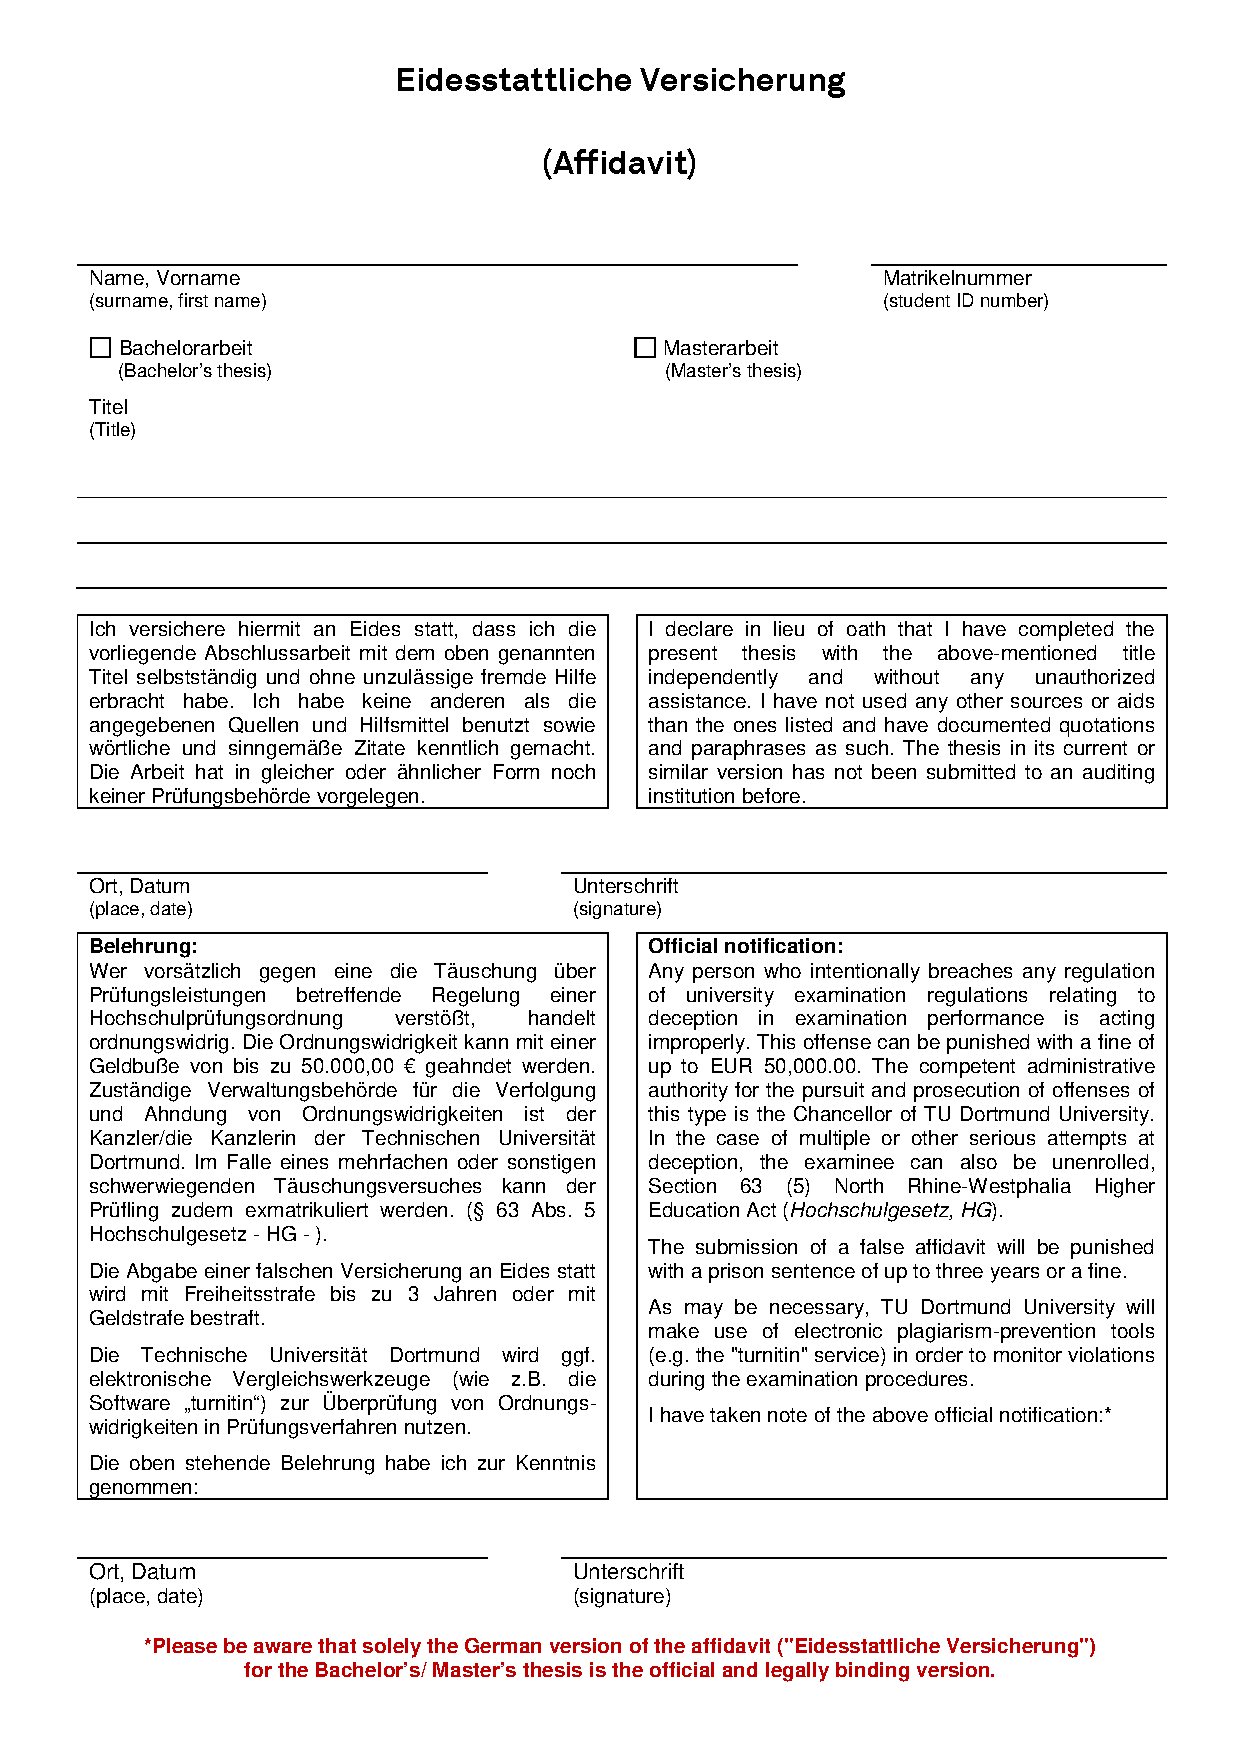
\includepdf[pages={1}]{resources/Eidesstattliche_Versicherung.pdf}

% Bibliografie im .bib Format einfügen


\end{document}